\documentclass[tikz,border=5pt]{standalone}
\usepackage{amsmath}
\usetikzlibrary{arrows.meta,positioning,fit,backgrounds}

\begin{document}
\hyphenpenalty=10000
\exhyphenpenalty=10000
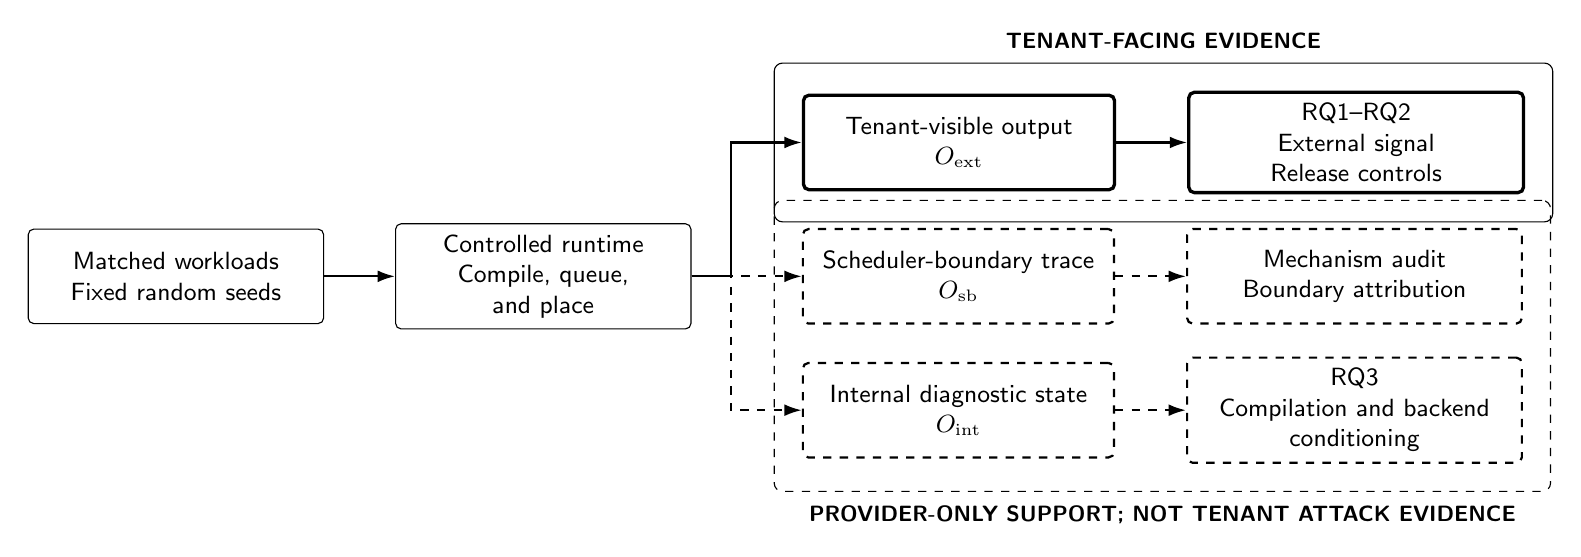
\begin{tikzpicture}[
  font=\sffamily\small,
  node distance=8mm and 9mm,
  stage/.style={draw=black, rounded corners=2pt, align=center,
    minimum height=12mm, text width=34mm, inner xsep=5pt,
    inner ysep=4pt, fill=white},
  view/.style={stage, text width=36mm},
  result/.style={stage, text width=39mm},
  tenant/.style={view, very thick},
  tenantresult/.style={result, very thick},
  provider/.style={view, dashed, thick},
  providerresult/.style={result, dashed, thick},
  flow/.style={-{Latex[length=2.2mm,width=1.5mm]}, thick},
  support/.style={flow, dashed},
  lane/.style={font=\sffamily\footnotesize\bfseries, fill=white, inner sep=2pt}
]

\node[stage] (inputs) {Matched workloads\\Fixed random seeds};
\node[stage, right=of inputs] (runtime) {Controlled runtime\\Compile, queue, and place};

\node[tenant, right=14mm of runtime, yshift=17mm] (ext)
  {Tenant-visible output\\$O_{\mathrm{ext}}$};
\node[tenantresult, right=of ext] (rq12)
  {RQ1--RQ2\\External signal\\Release controls};

\node[provider, right=14mm of runtime] (sb)
  {Scheduler-boundary trace\\$O_{\mathrm{sb}}$};
\node[providerresult, right=of sb] (audit)
  {Mechanism audit\\Boundary attribution};

\node[provider, right=14mm of runtime, yshift=-17mm] (int)
  {Internal diagnostic state\\$O_{\mathrm{int}}$};
\node[providerresult, right=of int] (rq3)
  {RQ3\\Compilation and backend\\conditioning};

\draw[flow] (inputs) -- (runtime);
\draw[flow] (runtime.east) -- ++(5mm,0) |- (ext.west);
\draw[support] (runtime.east) -- (sb.west);
\draw[support] (runtime.east) -- ++(5mm,0) |- (int.west);
\draw[flow] (ext) -- (rq12);
\draw[support] (sb) -- (audit);
\draw[support] (int) -- (rq3);

\begin{scope}[on background layer]
  \node[draw=black, rounded corners=3pt, fit=(ext)(rq12), inner sep=3.5mm] (tenantbox) {};
  \node[draw=black, dashed, rounded corners=3pt,
    fit=(sb)(audit)(int)(rq3), inner sep=3.5mm] (providerbox) {};
\end{scope}
\node[lane, above=1mm of tenantbox.north] {TENANT-FACING EVIDENCE};
\node[lane, below=1mm of providerbox.south]
  {PROVIDER-ONLY SUPPORT; NOT TENANT ATTACK EVIDENCE};

\end{tikzpicture}
\end{document}
